\documentclass[10pt]{mypackage}

% sans serif font:
%\usepackage{cmbright}
%\usepackage{sfmath}
%\usepackage{bbold} %better blackboard bold

%serif font + different blackboard bold for serif font
\usepackage{newpxtext,eulerpx}
\renewcommand*{\mathbb}[1]{\varmathbb{#1}}
\renewcommand*{\hbar}{\hslash}

\pagestyle{fancy} %better headers
\fancyhf{}
\rhead{Avinash Iyer}
\lhead{Ordinary Differential Equations: Homework 10}

\setcounter{secnumdepth}{0}

\begin{document}
\RaggedRight
\section{Part 1}%
\subsection{3.4, Problem 3}%
\begin{enumerate}[(a)]
  \item Solving the eigenvalues, we find
    \begin{align*}
      \det \begin{pmatrix}-\lambda & 2 \\ -2 & -\lambda\end{pmatrix} &= \lambda^2 + 4,
    \end{align*}
    so the eigenvalues are $\lambda = \pm 2i$.
  \item The origin is thus a center as each eigenvalue is pure imaginary.
  \item Since
    \begin{align*}
      e^{2it} &= \cos \left(2t\right) + i\sin \left(2t\right),
    \end{align*}
    we have that the period of each oscillation is $\pi$ and the frequency is $\frac{1}{\pi}$.
  \item Solving for the eigenvectors, we have
    \begin{align*}
      \begin{pmatrix}0 & 2 \\ -2 & 0\end{pmatrix} \begin{pmatrix}x\\y\end{pmatrix} &= 2i \begin{pmatrix}x\\y\end{pmatrix}\\
      2y &= 2ix\\
      y &= ix\\
      \vec{v}_1 &= \begin{pmatrix}1\\i\end{pmatrix}\\
      \vec{v}_2 &= \begin{pmatrix}1\\-i\end{pmatrix}\\
      \vec{Y}(t) &= \left(\cos \left(2t\right) + i\sin \left(2t\right)\right) \begin{pmatrix}1\\i\end{pmatrix}\\
                 &= \begin{pmatrix}\cos\left(2t\right)\\-\sin\left(2t\right)\end{pmatrix} + i\begin{pmatrix}\sin\left(2t\right)\cos\left(2t\right)\end{pmatrix}\\
      \vec{Y}_1(t) &= \begin{pmatrix}k_1\cos\left(2t\right) + k_2\sin\left(2t\right) \\ -k_1\sin\left(2t\right) + k_2\cos\left(2t\right)\end{pmatrix}.
    \end{align*}
    Solving the initial condition, we get $k_1 = 1$ and $k_2 = 0$, so our solution must be counterclockwise.
  \item\hfill
    \begin{center}
      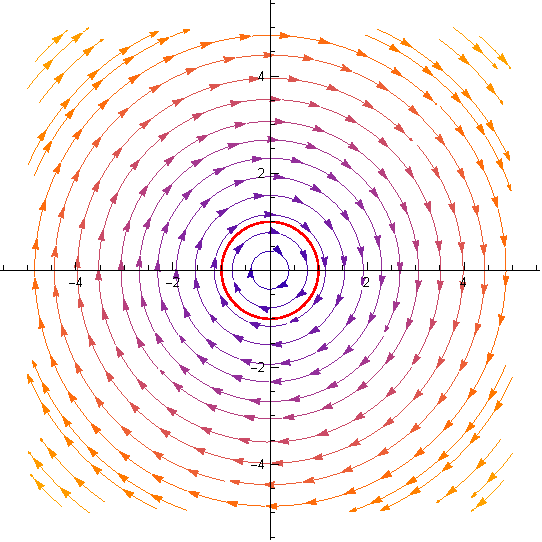
\includegraphics[width=7cm]{images/3_4_3e1.pdf} 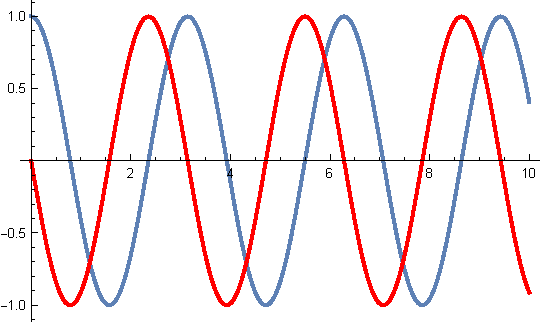
\includegraphics[width=7cm]{images/3_4_3e2.pdf}
    \end{center}
\end{enumerate}
\subsection{3.4, Problem 4}%
\begin{enumerate}[(a)]
  \item Solving the eigenvalues, we find
    \begin{align*}
      \det \begin{pmatrix}2-\lambda & 2 \\ -4 & 6-\lambda\end{pmatrix} &= \left(\lambda^2 - 8 \lambda + 12\right) + 8\\
      \lambda^2 - 8\lambda + 20 &= 0\\
      \lambda &= 4 \pm 2i.
    \end{align*}
  \item The origin is a spiral source as the real part of $\lambda$ is positive.
  \item The period of the oscillations is $\pi$, while the frequency is $\frac{1}{\pi}$.
  \item Finding the eigenvectors, we take
    \begin{align*}
      \begin{pmatrix}2 & 2 \\ -4 & 6\end{pmatrix} \begin{pmatrix}x\\y\end{pmatrix} &= \left(4+2i\right) \begin{pmatrix}x\\y\end{pmatrix}\\
      2x + 2y &= \left(4+2i\right)x\\
      2y &= \left(2+2i\right)x\\
      y &= \left(1+i\right)x\\
      \vec{v} &= \begin{pmatrix}1\\1+i\end{pmatrix}\\
      \vec{Y}(t) &= e^{4t}\left(\cos\left(2t\right) + i\sin\left(2t\right)\right) \begin{pmatrix}1\\1+i\end{pmatrix}\\
                 &= e^{4t} \begin{pmatrix}\cos\left(2t\right) + i\sin\left(2t\right) \\ \left(\cos\left(2t\right) + i\sin\left(2t\right)\right) + i\cos\left(2t\right) - \sin\left(2t\right)\end{pmatrix}\\
                 &= e^{4t} \begin{pmatrix}\cos\left(2t\right)\\ \cos\left(2t\right) - \sin\left(2t\right)\end{pmatrix} + ie^{4t} \begin{pmatrix}\sin\left(2t\right) \\ \cos\left(2t\right) + \sin\left(2t\right)\end{pmatrix}.
    \end{align*}
    Thus, our general solution is
    \begin{align*}
      \vec{Y}_1(t) &= e^{4t} \left(k_1\begin{pmatrix}\cos\left(2t\right) \\ \cos\left(2t\right) - \sin\left(2t\right)\end{pmatrix} + k_2 \begin{pmatrix}\sin\left(2t\right) \\ \cos\left(2t\right) + \sin\left(2t\right)\end{pmatrix}\right).
      \end{align*}
      With the initial condition of $\vec{Y}_0 = \begin{pmatrix}1\\1\end{pmatrix}$, we get $k_1 = k_2 = 1$. We find that the oscillations go clockwise.
    \item \hfill
      \begin{center}
        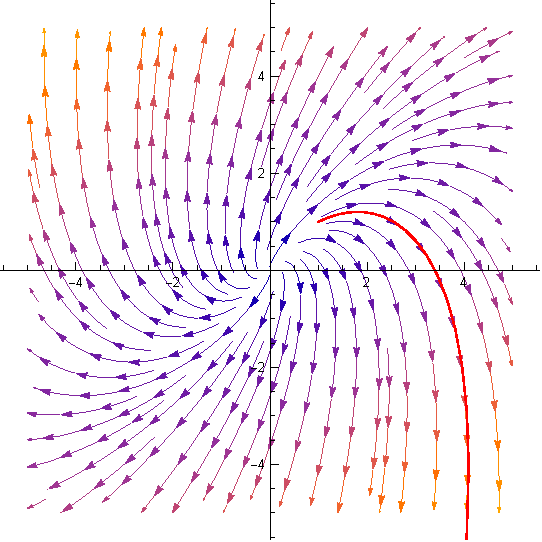
\includegraphics[width=7cm]{images/3_4_4e1.pdf} 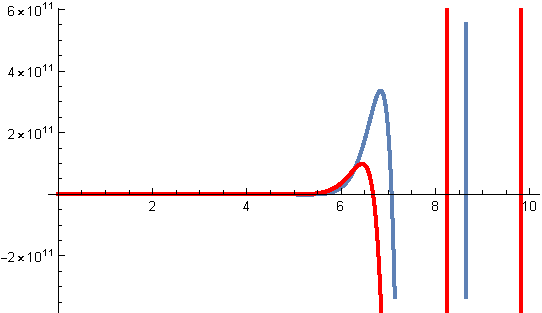
\includegraphics[width=7cm]{images/3_4_4e2.pdf}
      \end{center}
\end{enumerate}
\subsection{3.4, Problem 16}%
\begin{align*}
  \det \begin{pmatrix}a-\lambda & b \\ -b & a-\lambda\end{pmatrix} &= \left(\lambda - a\right)^2 + b^2\\
  \lambda &= a \pm \sqrt{-b^2}.
\end{align*}
Thus, $\lambda\in \C$.
\subsection{3.4, Problem 23}%
\begin{enumerate}[(a)]
  \item Let $v = \diff{y}{t}$. Then, we have
    \begin{align*}
      \diff{y}{t} &= v\\
      \diff{v}{t} &= -qy-pv.
    \end{align*}
  \item The matrix is
    \begin{align*}
      A &= \begin{pmatrix}0 & 1 \\ -q & -p\end{pmatrix},
    \end{align*}
    meaning that for complex eigenvalues, we must have, for
    \begin{align*}
      \lambda^2 - p\lambda + q &= 0,
    \end{align*}
    that $q > \frac{p^2}{4}$.
  \item If $p > 0$, and $q  > \frac{p^2}{4}$, then the origin is a spiral source. If $p < 0$ and $q > \frac{p^2}{4}$, then the origin is a spiral sink. If $p = 0$ and $q > 0$, then the origin is a center.
  \item I don't know how to do this problem.
\end{enumerate}
\subsection{3.5, Problem 3}%
\begin{enumerate}[(a)]
  \item The eigenvalue is found by
    \begin{align*}
      \lambda^2 + 6 \lambda + 9 &= 0\\
      \lambda &= -3.
    \end{align*}
  \item An eigenvector is
    \begin{align*}
      \vec{v} &= \begin{pmatrix}1\\1\end{pmatrix}.
    \end{align*}
  \item \hfill
    \begin{center}
      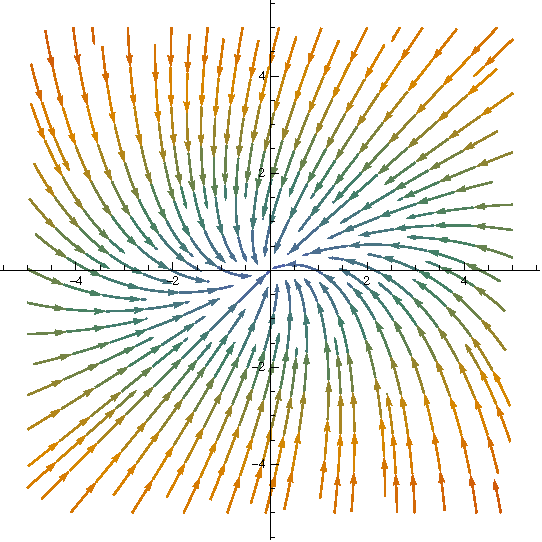
\includegraphics[width=10cm]{images/3_5_3c.pdf}
    \end{center}
  \item \hfill
    \begin{center}
      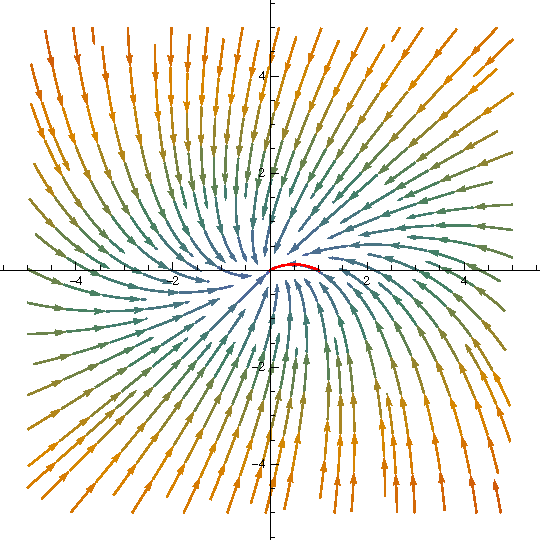
\includegraphics[width=10cm]{images/3_5_3d.pdf}
    \end{center}
  \item \hfill
    \begin{center}
      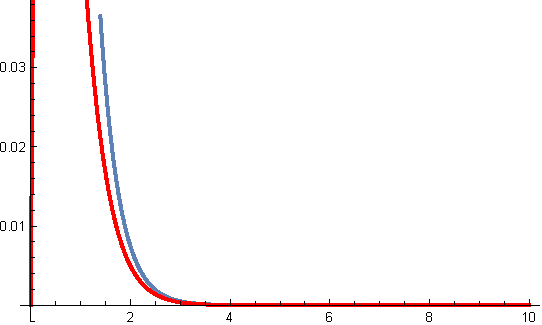
\includegraphics[width=10cm]{images/3_5_3e.pdf}
    \end{center}
\end{enumerate}
\subsection{3.5, Problem 4}%
\begin{enumerate}[(a)]
  \item The eigenvalue is found by
    \begin{align*}
      \lambda\left(\lambda + 2\right) + 1 &= 0\\
      \lambda^2 + 2\lambda + 1 &= 0\\
      \lambda &= -1.
    \end{align*}
  \item An eigenvector is
    \begin{align*}
      y &= -x\\
      \vec{v} &= \begin{pmatrix}1\\-1\end{pmatrix}.
    \end{align*}
  \item \hfill
    \begin{center}
      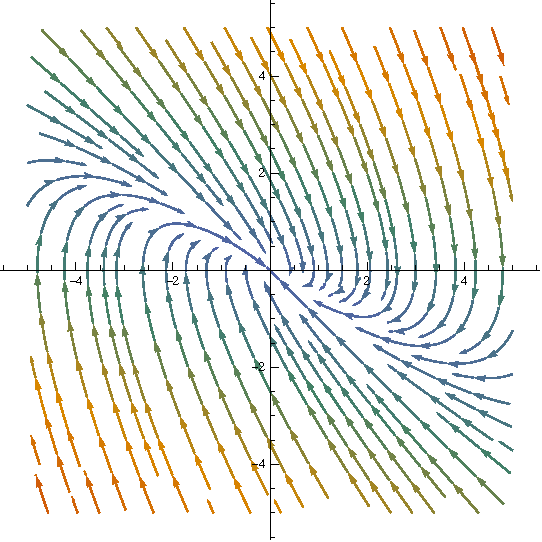
\includegraphics[width=10cm]{images/3_5_4c.pdf}
    \end{center}
  \item \hfill
    \begin{center}
      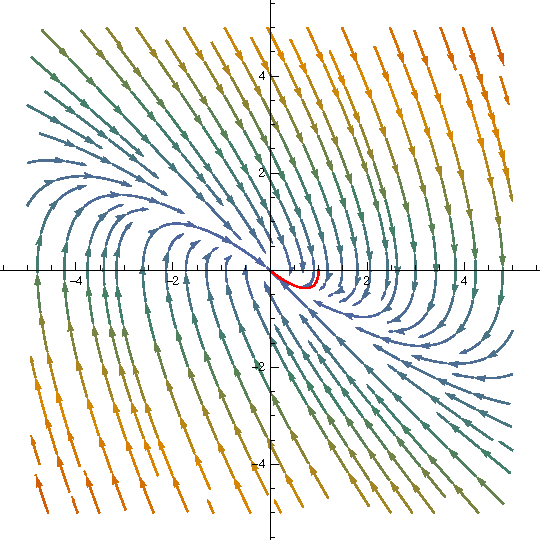
\includegraphics[width=10cm]{images/3_5_4d.pdf}
    \end{center}
  \item \hfill
    \begin{center}
      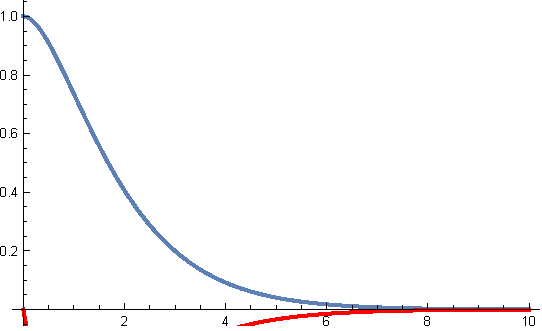
\includegraphics[width=10cm]{images/3_5_4e.pdf}
    \end{center}
\end{enumerate}
\subsection{3.5, Problem 7}%
\begin{enumerate}[(a)]
  \item We find the eigenvalue to be
    \begin{align*}
      \lambda &= -3,
    \end{align*}
    with corresponding eigenvector
    \begin{align*}
      \vec{v} &= \begin{pmatrix}-1\\1\end{pmatrix}.
    \end{align*}
    The general solution is, thus,
    \begin{align*}
      \vec{Y}(t) &= te^{-t} \begin{pmatrix}-x_0 - y_0 \\ x_0-3y_0\end{pmatrix} + e^{-t} \begin{pmatrix}x_0\\y_0\end{pmatrix}.
    \end{align*}
  \item With initial condition $\vec{Y}(0) = \begin{pmatrix}1\\0\end{pmatrix}$, we have
    \begin{align*}
      \vec{Y}(t) &= te^{-t} \begin{pmatrix}-1\\1\end{pmatrix} + e^{_t} \begin{pmatrix}1\\0\end{pmatrix}.
    \end{align*}
  \item \hfill
    \begin{center}
      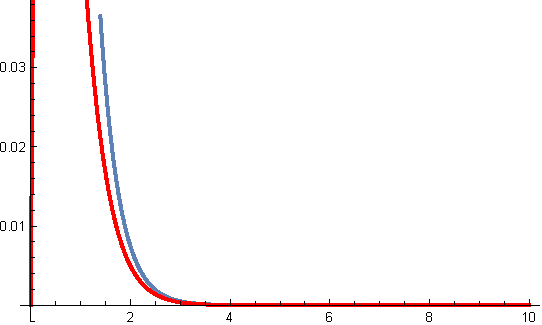
\includegraphics[width=10cm]{images/3_5_7c.pdf}
    \end{center}
\end{enumerate}
\subsection{3.5, Problem 9}%
\begin{enumerate}[(a)]
  \item If $\beta = \frac{\alpha^2}{4}$, then the quadratic has a double root.
  \item If $\beta = 0$, then the quadratic has zero as a root.
\end{enumerate}
\subsection{3.5, Problem 10}
\begin{enumerate}[(a)]
  \item If $\lambda > 0$, then $\lim_{t\rightarrow\infty}te^{\lambda t} = \infty$, as both $t$ and $e^{\lambda t}$ are positive.
  \item If $\lambda < 0$, then $\lim_{t\rightarrow\infty}te^{\lambda t} = 0$ as, while $t > 0$, $e^{\lambda t}$ decreases at a faster rate than $t$ increases.
\end{enumerate}
\end{document}
